\begin{frame}
\frametitle{\darkhighlightiii{Introduction: l'inverse canonique}}
\framesubtitle{Vers une définition typologique de l'opposition direct/inverse}
%\pause
\begin{wideitemize}
\item Le direct/inverse fait partie des types de marquages de
  l'alignement
\begin{smallwideitemize}
\item un des marquages des systèmes d'alignement hiérarchique
\item autres alignements: accusatif, ergatif, neutre, tripartite
\pause
\item le plus souvent un marquage morphologique sur le verbe
\item indexation des deux arguments pour les verbes transitifs
\item symétrie entre formes:\\ exemple: identité formelle pour les formes \textsc{1sg>3sg} et
  \textsc{3sg>1sg}\\ à un \textsc{marqueur d'inverse} près
\pause
\item phénomène typologique moins connu
\item \cite{zuniga06}
%\pause
\end{smallwideitemize}
\end{wideitemize}
\end{frame}


\begin{frame}
\frametitle{\darkhighlightiii{Introduction: l'inverse canonique}}
\framesubtitle{La distribution des types d'alignements 
  dans le monde (carte du WALS)}
\begin{center}
\vspace*{-.3cm}
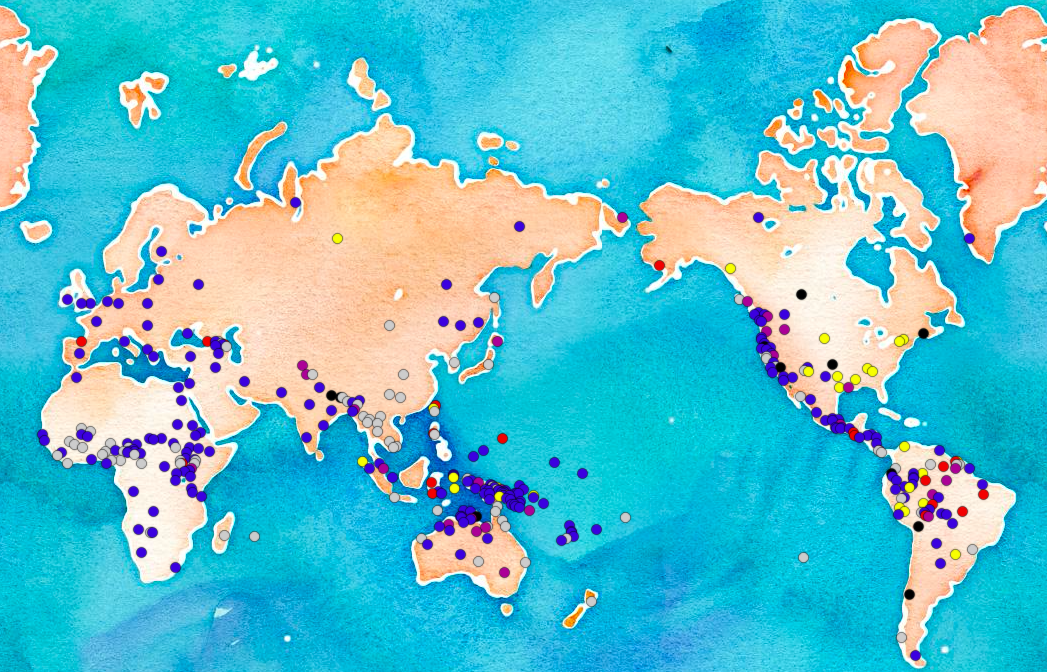
\includegraphics[width=120mm]{hierarchy}

\end{center}
\end{frame}


\begin{frame}
\frametitle{\darkhighlightiii{Introduction: l'inverse canonique}}
\framesubtitle{La distribution des langues à marquage hiérarchique
  sur le verbe (carte du WALS)}
\begin{center}
\vspace*{-.3cm}
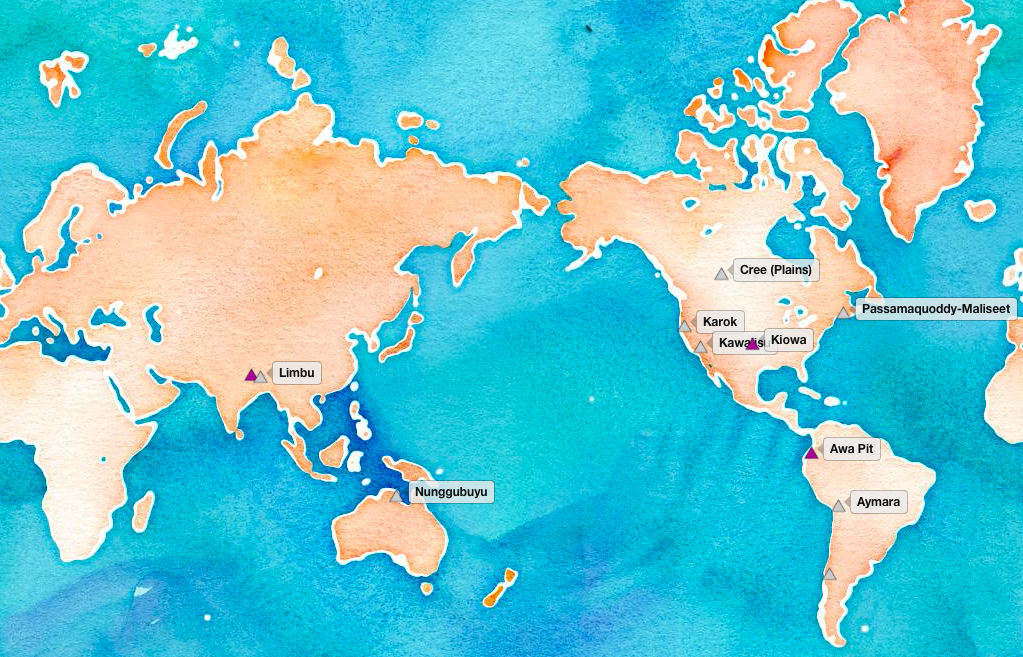
\includegraphics[width=120mm]{hierarchy-marking}

\end{center}
\end{frame}

\begin{frame}
\frametitle{\darkhighlightiii{Introduction: l'inverse canonique}}
\framesubtitle{Vers une définition typologique de l'opposition direct/inverse}
%\pause
\begin{wideitemize}
\item Un nombre non-négligeable de langues est considéré comme affichant un marquage de
  type direct/inverse
%\begin{smallwideitemize}
\item Mais la réalisation du direct/inverse varie en fait de façon
  considérable dans ces langues\\ 
\item[\highlighti{\lefthand}] Besoin d'une approche typologique du phénomène
%\end{smallwideitemize}
\end{wideitemize}
%\item But d'une approche typologique
\begin{wideitemize}
%\begin{smallwideitemize}
\item[\highlightiv{\lefthand}]~Mise en place d'un système de notions fonctionnel
\item[\highlightiv{\lefthand}] approche canonique
%\end{smallwideitemize}
\end{wideitemize}
\begin{wideitemize}
\item[\highlightii{\lefthand}] But de ce papier {\ra} proposer une définition typologiquement
  fonctionnelle des systèmes à direct/inverse
\end{wideitemize}
\end{frame}